\subsection{Schritt 1 - Formular in Grundstruktur erstellen}

Im ersten Schritt soll die Formular-Anwendung in ihrer Grundstruktur entwickelt werden.  Das beinhaltet alle drei Oberflächen, welche in den darauf folgenden Schritten lediglich erweitert werden.  Das Formular erhält noch keine  Validierung. Somit sind alle Eingaben oder nicht kompatible Selektionen erlaubt.Die erste Ansicht, welche der Benutzer sieht, soll die Übersicht der bereits eingetragenen Maßnahmen sein \Abb{\ref{fig:Schritt1Uebersicht}}.

% TODO: rausgekürzt, doch wieder rein nehmen?
%Dort ist auch zu sehen, dass die Anwendung ohne Anpassungen zunächst einmal im sogenannten Material Design\footnoteI{Material Design umfasst eine Reihe von Prinzipien zur Auszeichnung von Benutzeroberflächen. Das ist Design-System wurde von Google Inc. entwickelt.  Der Name leitet sich daher ab, dass Objekte mit der Nachahmung physikalischer Eigenschaften - wie etwa dem Werfen eines Schattens - den Eindruck von tatsächlichen Materialien erwecken. \footnote{\cite{MaterialDesignIntroduction}}} gestylt ist.
\begin{figure}[H]
  \centering
  \includegraphics[width=1.0\textwidth]{Inhalt/Hauptteil/Implementierung/Schritt-1/Übersicht.png}
  \caption[Schritt 1 Übersicht]{Der Übersicht-Bildschirm zeigt in  Schritt 1 zunächst nur die Maßnahmen mit ihrem Titel und Bearbeitungsdatum in den Kategorien \enquote{Abgeschlossen} und \enquote{In Bearbeitung}. Quelle: Eigene Abbildung}
  \label{fig:Schritt1Uebersicht}
\end{figure}
Die Auflistung der Maßnahmen erfolgt in den Kategorien \enquote{In Bearbeitung} und \enquote{Abgeschlossen}. Innerhalb dieser Rubriken werden die Maßnahmen in einer Tabelle angezeigt. Mit einem Klick auf den Button unten rechts im Bild wird der Benutzer auf die zweite Ansicht weitergeleitet: die Eingabemaske \Abb{\ref{fig:Schritt1Eingabemaske}}.
\begin{figure}[H]
  \centering
  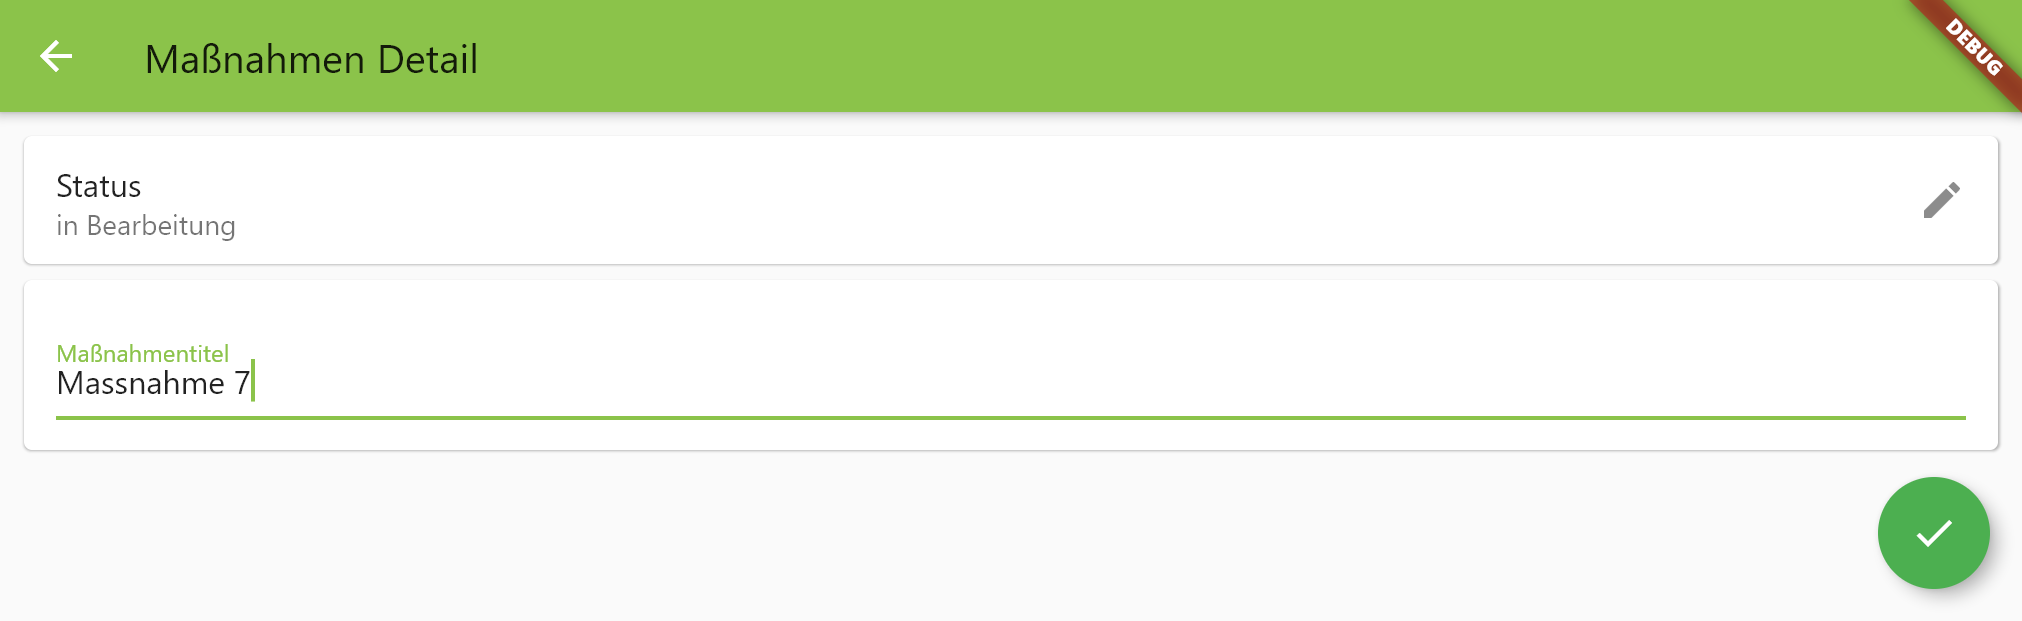
\includegraphics[width=1.0\textwidth]{Inhalt/Hauptteil/Implementierung/Schritt-1/Eingabemaske.png}
  \caption[Schritt 1 Eingabemaske]{Die Eingabemaske zeigt im Schritt 1 eine Karte zum Selektieren des Status und ein Eingabefeld für den Titel. Quelle: Eigene Abbildung}
  \label{fig:Schritt1Eingabemaske}
\end{figure}
Sie ermöglicht die Eingabe des Maßnahmen-Titels über ein simples Eingabefeld. Darüber hinaus ist die Selektions-Karte für den Status zu sehen. Mit einem Klick auf diese Karte öffnet sich der Selektions-Bildschirm. Er ermöglicht die Auswahl der Auswahloptionen, in diesem Fall die Optionen \enquote{in Bearbeitung} und \enquote{abgeschlossen}
\Abb{\ref{fig:Schritt1SelektionsBildschirmStatus}}.

\begin{figure}[H]
  \centering
  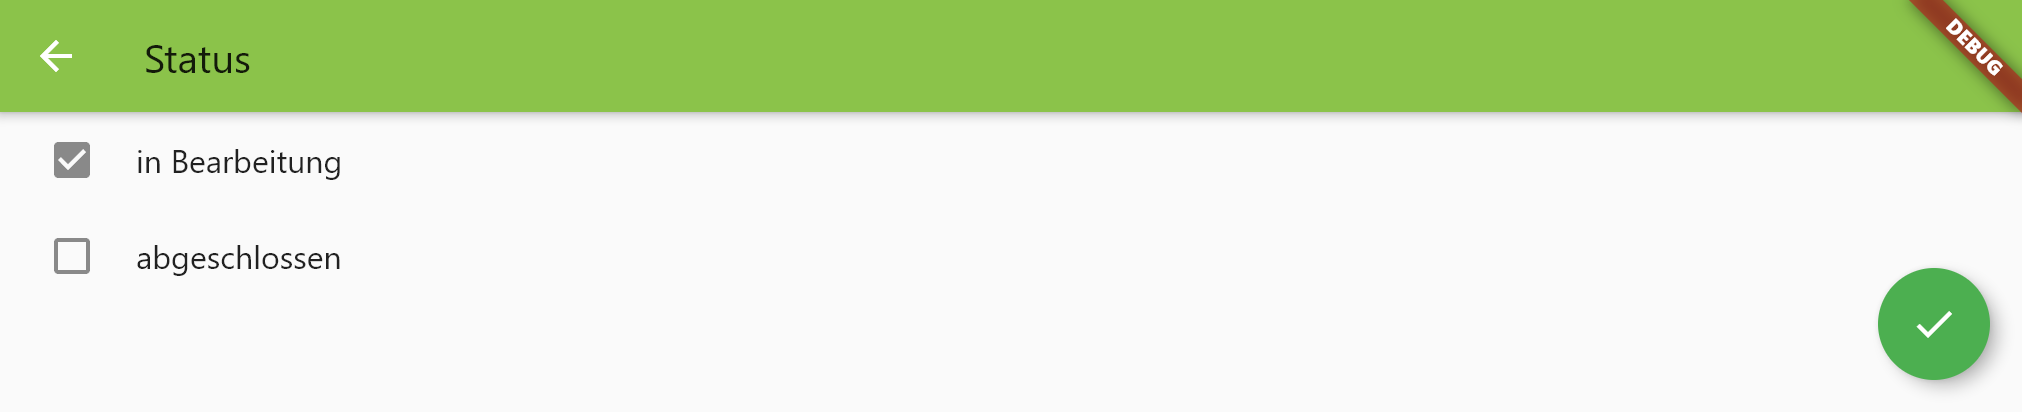
\includegraphics[width=1.0\textwidth]{Inhalt/Hauptteil/Implementierung/Schritt-1/Status Auswahl.png}
  \caption[Schritt 1 Selektions-Bildschirm für Status]{Der Selektions-Bildschirm für das Feld Status erlaubt die Auswahl der Optionen \enquote{in Bearbeitung} und \enquote{abgeschlossen}. Quelle: Eigene Abbildung}
  \label{fig:Schritt1SelektionsBildschirmStatus}
\end{figure}

% TODO: rausgekürzt, doch wieder rein nehmen?
%\footnoteI{Ein floating action button (FAB) ist im Material Design ein Button, der über der Benutzeroberfläche schwebt und daher dem Benutzer leicht ins Auge fällt. Aus diesem Grund wird er für primäre Aktionen genutzt - in diesem Fall dem Erstellen einer neuen Maßnahme. \footnote{\cite{MaterialDesignFloatingActionButton}}} ist in der unteren rechten Ecke der Ansicht zu finden. Mit einem Klick darauf wird der Benutzer auf die zweite Ansicht weitergeleitet: die Eingabemaske. 

\subsubsection{Auswahloptionen hinzufügen}

Dart verfügt – anders als beispielsweise Java\footcite[Vgl.][S. 321]{TheJavaLanguageSpecificationJavaSE16Edition} – nicht über Aufzählungstypen mit zusätzlichen Eigenschaften. Das Schlüsselwort \mintinline{dart}{enum} in Dart erlaubt lediglich die Auflistung konstanter Symbole\footcite[Vgl.][S. 74f.]{DartProgrammingLanguageSpecification5thedition}. Für die Auswahl Optionen ist es jedoch notwendig, dass es zwei Eigenschaften gibt:
\begin{itemize}
  \parsep 0pt
  \topsep 0pt
  \itemsep 0pt 

  \item die Abkürzung, die in der resultierendem Datei gespeichert werden soll
  \item und der Beschreibungstext, welcher in der Oberfläche angezeigt wird.
\end{itemize}
Das hat den Hintergrund, dass die Abkürzungen weniger Speicherplatz einnehmen und die Beschreibung sich in Zukunft auch ändern darf. Würde anstatt der Abkürzung die Beschreibung als Schlüssel verwendet werden, so würde eine Datei, die mit einer älteren Version des Formulars erstellt wurde, nicht mehr von neueren Versionen der Applikationeingelesen werden können. Der alte Beschreibungstext würde nicht mehr mit dem Text übereinstimmen, der als Schlüssel in der Anwendung verwendet wird. 


Die beiden Zustände \enquote{in Bearbeitung} und \enquote{abgeschlossen} werden daher in Listing \ref{Schritt1KlasseLetzterStatus} als statische Klassenvariablen deklariert \Z{6-7}. Die beiden Konstruktor-Aufrufe übergeben dabei als erstes Argument die Abkürzung und als zweites Argument die Beschreibung. Der Konstruktor selbst \Z{9-10} deklariert die beiden Parameter als positionale Parameter.

\begin{alexlisting}{Schritt 1}{Die Klasse LetzterStatus}
  {Quellcode/Schritt-1/conditional_form/lib/choices/choices.dart}
  {firstline=5, lastline=11}
  \label{lst:Schritt1KlasseLetzterStatus}
\end{alexlisting}

\paragraph{Positionale Parameter}

Im Vergleich zu den benannten Parametern ist bei den positionalen Parametern nur ihre Reihenfolge in der Parameterliste ausschlaggebend. Das Argument für die \IC{abbreviation} steht dabei also immer an erster Stelle und das Argument für \IC{description} immer an der zweiten \Z{6-7}. Positionale Parameter sind vorgeschrieben. Werden sie ausgelassen, so gibt es einen Compilerfehler. \DartSpec{74f.}

Die Klasse \IC{LetzterStatus} erbt von der Klasse \IC{Choice} \Z{5}. Der Konstruktor der Klasse \Z{7} übergibt beide Parameter als Argumente an den Konstruktor der Klasse \IC{Choice}. Weil das Aufrufen des sogenannten Super-Konstruktors zum statischen Teil der Objekt-Instanziierung gehört, muss der Aufruf von \IC{super} in der Initialisierungsliste erfolgen. Die Initialisierungsliste wird mit dem \IC{:} nach der Parameterliste eingeleitet \Z{10}\DartSpec{42}.

\begin{alexlisting}{Schritt 1}{Die Klasse Choice}
  {Quellcode/Schritt-1/conditional_form/lib/choices/base/choice.dart} 
  {firstline=3, lastline=7}
  \label{lst:Schritt1KlasseChoice}
\end{alexlisting}

Die Klasse \IC{Choice} \Lst{\ref{lst:Schritt1KlasseChoice}} deklariert lediglich die beiden Felder description und abbreviation jeweils als \IC{String} \Z{4-5}. Beide sind mit \IC{final} gekennzeichnet, was sie zu unveränderlichen Instanzvariablen macht. Nach der Initialisierung, können sie keine anderen Werte annehmen. \DartSpec{S16} Die Initialisierung der beiden Variablen muss im statischen Kontext der Instanziierung erfolgen. Mit der abgekürzten Schreibweise \IC{this.abbreviation} und \IC{this.description} im Konstruktor \Z{7} werden die Parameter den Feldern zugewiesen. Dies erübrigt die Zuweisung die man Ansonstenin der Form \IC{this.abbreviation = abbreviation} und \IC{this.description = description} in der Initialisierungsliste erreichen würde\DartSpec{40f}.
% Auch String description wird gespart






\begin{alexlisting}{Schritt 1}{Die Menge letzterStatusChoices}
  {Quellcode/Schritt-1/conditional_form/lib/choices/choices.dart}
  {firstline=13}
  \label{lst:Schritt1DieMengeLetzterStatusChoices}
\end{alexlisting}

\begin{alexlisting}{Schritt 1}{Die Klasse Choices}
  {Quellcode/Schritt-1/conditional_form/lib/choices/base/choice.dart}
  {firstline=10}
  \label{lst:Schritt1KlasseChoices}
\end{alexlisting}

\begin{listing}[h]
  \begin{minted}[firstnumber=6]{dart}
part '$file_name$.g.dart';

abstract class $ClassName$ implements Built<$ClassName$, $ClassName$Builder> {
    $todo$
    
    $ClassName$._();
    factory $ClassName$([void Function($ClassName$Builder) updates]) = _$$$ClassName$;
}
\end{minted}
  \caption[built_value Live Template]{Live Template für die Erstellung von built_value Boilerplate-Code in Android Studio, Quelle: Jetbrains Marketplace Built Value Snippets Plugin}
  \label{lst:BuiltValueLiveTemplate}
\end{listing}


\section{Ein Test soll verifizieren, dass die Daten korrekt abgelegt werden}



Doch damit die Daten angezeigt und verändert werden können, müssen sie zunächst serialisierbar sein, sodass sie auf einen Datenträger geschrieben und von dort auch wieder gelesen werden können.
% todo: Serialisierung erklären
Die zwei bekanntesten Bibliotheken zum Serialisieren in Dart heißen json_serializable und built_value.
% todo medium: Vgl. https://flutter.dev/docs/development/data-and-backend/json
% todo medium: Was ist flutter, Flutter nutzt Dart
% todo medium: Model View View Model
Beide haben gemeinsam, dass sie Quellcode generieren, welcher die Umwandlung der Objekte in JSON übernimmt.
% todo: json_serializable erklären
% todo: tree shaking erklären https://flutter.dev/docs/development/data-and-backend/json
built_value bietet im Gegensatz zu JSON Serializable jedoch die Möglichkeit unveränderbare Werte-Typen -  sogenannte immutable value types -  zu erstellen. Da diese  unveränderbaren Werte noch bei der Erstellung des sogenannten ViewModels -  Mehr dazu im Kapitel XXX - hilfreich werden, wurde sich für diese Bibliothek entschieden.
% todo high: Kapitel Referenz einfügen

Ein Werte-Typ für built_value erfordert etwas Boilerplate-Code,  um den generierten Quellcode mit der selbstgeschriebenen Klasse zu verknüpfen.  Dieser Boilerplate-Code kann durch das Live Template für Android Studio in Listing \ref{lst:BuiltValueLiveTemplate} generiert werden. \footnoteL{https://web.archive.org/web/20210710140113/https://github.com/GiancarloCode/built-value-snippets/blob/master/intellij/src/main/resources/liveTemplates/snippets.xml}
% todo medium: live template erklären






\$ClassName\$ Wird dabei jeweils durch den gewünschten Klassennamen ersetzt. Android Studio erlaubt, dass bei Einfügen des live Templates der Klassenname einmalig eingegeben werden muss.  Anschließend wird mithilfe des Templates der Boilerplate Code generiert. In Listing \ref{lst:Schritt1WerteTypMassnahme} ist der Werte-Typ \enquote{Maßnahme} zu sehen. Die Zeilen 11 bis 13, sowie 23 bis 28 wurden dabei automatisch erstellt. Die Zeilen 14 bis 21 wurden hinzugefügt. Zunächst soll die Maßnahme über die \enquote{guid} - Kurzform von General Unique Identifier - eindeutig identifiziert werden können.
%  todo - guid General unique identifier erklären
Die Attribute \enquote{letzteBearbeitung} und \enquote{identifikatoren} sind im Gegensatz zu dem String-Attribut guid zusammengesetzte Datentypen, die im Folgenden weiter beleuchtet werden.

Auffällig ist, dass es sich hier um eine abstrakte Klasse handelt und die drei Attribute jeweils Getter-Methoden ohne Implementierung sind. Eine solche Getter-Methode speichert keinen wert, sondern gibt lediglich den Wert eines Feldes zurück. Die dazugehörigen Felder,  Setter-Methoden, die konkrete Klasse und der restliche generierte Code ist in der gleichnamigen Datei mit der Endung \enquote{.g.dart} (Zeile 11) zu finden.

Die Klassen-Methode \enquote{_initializeBuilder} kann in jedem Werte-Typ hinterlegt werden, um Standardwerte für Felder festzulegen.
% todo medium: Vgl. https://pub.dev/packages/built_value/changelog
Die Methode wird intern von built_value aufgerufen. Bei dem Feld \enquote{guid} handelt es sich um einen String, der keine Null-Werte zulässt. Könnte das Feld auch Null-Werte annehmen, so wäre die Notation in Dart dafür stattdessen \enquote{String? get guid;}. built_value erwartet also immer einen Wert für dieses Feld. Sollte die Datei gelesen werden, welche die Maßnahmen enthält, so enthält jede Maßnahme bei der Deserialisierung den abgespeicherten Wert für die \enquote{guid} und somit wird das Feld gefüllt. Doch sollte eine leere Maßnahme über einen Konstruktor erstellt werden, so wäre das Feld \enquote{guid} leer und built_value würde einen Fehler auslösen. Aus diesem Grund wird in der Zeile 21 für das Feld \enquote{guid} ein Standardwert festgelegt, nämlich eine zufällige  generierte ID die dem Standard Uuid der Version 4 entspricht.
% todo high:  https://www.ietf.org/rfc/rfc4122.txt
Die Attribute \enquote{letzteBearbeitung} und \enquote{identifikatoren} erhalten dagegen ganz automatisch Standardwerte in Form von Instanzen der dazugehörigen Klassen. Diese wiederum konfigurieren ihre eigenen Felder und deren initialwerte.

\begin{alexlisting}{Schritt 1}{Der Werte-Typ Massnahme}
  {Quellcode/Schritt-1/conditional_form/lib/data_model/massnahme.dart}
  {firstline=6, lastline=23}
  \label{lst:Schritt1WerteTypMassnahme}
\end{alexlisting}

Der Werte-Typ Identifikatoren ist in Listing \ref{lst:Schritt1WerteTypIdentifikatoren} zu sehen.  Er enthält das Attribut \enquote{massnahmenTitel}, welcher im Eingabeformular durch das Texteingabefeld gefüllt werden wird.

\begin{alexlisting}{Schritt 1}{Der Werte-Typ Identifikatoren}
  {Quellcode/Schritt-1/conditional_form/lib/data_model/massnahme.dart}
  {firstline=25, lastline=30}
  \label{lst:Schritt1WerteTypIdentifikatoren}
\end{alexlisting}

Schließlich enthält der Werte-Typ \enquote{LetzteBearbeitung} in Listing \ref{lst:Schritt1WerteTypLetzteBearbeitung} noch die Attribute \enquote{letztesBearbeitungsDatum} in Zeile 43 und \enquote{letzterStatus} in Zeile 50. Im Eingabeformular wird der Selektions-Bildschirm den Inhalt des Feldes \enquote{letzterStatus} Bestimmen. Der initiale Wert auf wird in Zeile 54 auf einen konstanten Wert gesetzt, der dem Zustand \enquote{in Bearbeitung} entspricht - mehr dazu im Kapitel CCCCCCCC.
% todo high: Kapitel Choices einfügen

Das Attribut \enquote{letztesBearbeitungsDatum} ist dagegen nicht im Formular änderbar, sondern wird einmalig in Zeile 53 auf den aktuellen Zeitstempel gesetzt. Zugehörig zu diesem Attribut gibt es noch eine abgeleitete Eigenschaft namens \enquote{formattedDate} (Zeilen 45-48).  Es ist eine Hilfsmethode, die das letzte Bearbeitungsdatum in ein für Menschen lesbares Datumsformat umwandelt. In dem Übersichts-Bildschirm Abbildung \ref{fig:Schritt1Uebersicht} ist das Datumsformat sichtbar.

Da diese Getter-Methode eine Implementierung besitzt, wird für sie von built_value kein Quellcode für die Serialisierung generiert.



\begin{alexlisting}{Schritt 1}{Der Werte-Typ LetzteBearbeitung}
  {Quellcode/Schritt-1/conditional_form/lib/data_model/massnahme.dart}
  {firstline=41, lastline=54}
  \label{lst:Schritt1WerteTypLetzteBearbeitung}
\end{alexlisting}


\begin{alexlisting}{Schritt 1}{Der Serialisierer für Massnahme und Storage}
  {Quellcode/Schritt-1/conditional_form/lib/data_model/serializers.dart}
  {firstline=10, lastline=12}
  \label{lst:Schritt1Serialisierer}
\end{alexlisting}



% Storage Klasse zeigen und beschreiben
% serializers Klasse zeigen und beschreiben
% Korrigieren (Unten)
Wird nun der Befehl \texttt{flutter pub run build_runner build} ausgeführt, so wird der Quellcode generiert und die Werte-Typen können für die Serialisierung genutzt werden.

Das Ergebnis der Serialisierung wird im dazugehörigen Unit-Test ersichtlich. Listing ZZZZZZZ zeig den Unit Test für den Typ Maßnahme.
In Zeile 8 wird ein Objekt der Klasse Massnahme instanzieiert. Anders als bei gewöhnlichen Datentypen lassen sich bei diesem unveränderlichen Datentyp keine Attribute nach der Erstellung anpassen. Die einzige Möglichkeit besteht darin, ein neues Objekt  mit dem gewünschten Attributwert zu erstellen und die  restlichen Werte des alten Objektes zu übernehmen.  dies ist in Bild Vaio mithilfe des sogenannten Bilder Entwurfsmuster möglich. In den Zeilen 9 bis 10 wird so ein neues Objekt von der Klasse Maßnahme mit Hilfe der Methode rebuild erzeugt und anschließend der Referenz Maßnahme zugewiesen, wodurch sie ihren alten Wert verliert.





\begin{alexlisting}{Schritt 1}{Ein automatisierter Testfall überprüft}
  {Quellcode/Schritt-1/conditional_form/test/data_model/massnahme_test.dart}
  {firstline=6, lastline=23}
  \label{lst:MaßnahmeSerialisiertOhneFehlerUnitTest}
\end{alexlisting}

\begin{alexlisting}{Schritt 1}{Ein automatisierter Testfall überprüft}
  {Quellcode/Schritt-1/conditional_form/test/data_model/massnahme_test.dart}
  {firstline=36, lastline=56}
  \label{lst:MaßnahmeDeserialisiertOhneFehlerUnitTest}
\end{alexlisting}





\begin{alexlisting}{Schritt 1}{Der Werte-Typ Storage}
  {Quellcode/Schritt-1/conditional_form/lib/data_model/storage.dart}
  {firstline=9, lastline=21}
  \label{lst:Schritt1WerteTypStorage}
\end{alexlisting}




\begin{alexlisting}{Schritt 1}{Ein automatisierter Testfall überprüft}
  {Quellcode/Schritt-1/conditional_form/test/data_model/storage_test.dart}
  {firstline=7, lastline=31}
  \label{lst:Schritt1MaßnahmenSerialisierenOhneFehlerUnitTest}
\end{alexlisting}



\begin{alexlisting}{Schritt 1}{Ein automatisierter Testfall überprüft}
  {Quellcode/Schritt-1/conditional_form/test/data_model/storage_test.dart}
  {firstline=48, lastline=74}
  \label{lst:Schritt1MaßnahmenDeserialisierenOhneFehlerUnitTest}
\end{alexlisting}





\begin{alexlisting}{Schritt 1}{Die Klasse MassnahmenJsonFile}
  {Quellcode/Schritt-1/conditional_form/lib/persistence/massnahmen_json_file.dart}
  {firstline=7, lastline=31}
  \label{lst:Schritt1KlasseMassnahmenJsonFile}
\end{alexlisting}

\begin{alexlisting}{Schritt 1}{Die Klasse MassnahmenPool}
  {Quellcode/Schritt-1/conditional_form/lib/data_access/massnahmen_pool.dart}
  {firstline=8}
  \label{lst:Schritt1KlasseMassnahmenPool}
\end{alexlisting}















\begin{listing}[htbp]
  \begin{minted}[firstnumber=13]{dart}
final createNewMassnahmeButtonKey = GlobalKey();

class MassnahmenMasterScreen extends StatelessWidget {
  static const routeName = '/massnahmen_master';

  const MassnahmenMasterScreen({Key? key}) : super(key: key);

  @override
  Widget build(BuildContext context) {
    final massnahmenPool = Provider.of<MassnahmenPool>(context, listen: false);

    return Scaffold(
      appBar: AppBar(
        title: const Text('Maßnahmen Master'),
      ),
      body: StreamBuilder<Storage>(
          stream: massnahmenPool.storageSubject,
          builder: (context, _) {
            return SingleChildScrollView(...);
          }),
      floatingActionButton: FloatingActionButton(
          key: createNewMassnahmeButtonKey,
          child: const Icon(
            Icons.post_add_outlined,
            color: Colors.white,
          ),
          onPressed: () {
            final vm =
                Provider.of<MassnahmenFormViewModel>(context, listen: false);

            vm.model = Massnahme();
            Navigator.of(context).pushNamed(MassnahmenDetailScreen.routeName);
          }),
    );
  }
}

\end{minted}
  \caption[Schritt 1 Klasse MassnahmenMasterScreen Struktur]{Die Struktur der Klasse MassnahmenMasterScreen, Quelle: Eigenes Listing, \newline Datei: Quellcode/Schritt-1/conditional_form/lib/screens/massnahmen_master.dart}

  \label{lst:Schritt1KlasseMassnahmenMasterScreenStruktur}
\end{listing}



\begin{listing}[htbp]
  \begin{minted}[firstnumber=31]{dart}
return SingleChildScrollView(
  child: Column(
    crossAxisAlignment: CrossAxisAlignment.start,
    children: [
      const Padding(
        padding: EdgeInsets.all(16.0),
        child: Text(
          "Abgeschlossen",
          style: TextStyle(fontSize: 20),
        ),
      ),
      SingleChildScrollView(
          scrollDirection: Axis.horizontal,
          child: Padding(
            padding: const EdgeInsets.all(16.0),
            child: MassnahmenTable(
                massnahmenPool.storage.massnahmen
                    .where((m) =>
                        m.letzteBearbeitung.letzterStatus ==
                        LetzterStatus.fertig.abbreviation)
                    .toSet(), onSelect: (selectedMassnahme) {
              final vm = Provider.of<MassnahmenFormViewModel>(
                  context,
                  listen: false);
              vm.model = selectedMassnahme.rebuild((m) => m
                ..letzteBearbeitung.letztesBearbeitungsDatum =
                    DateTime.now().toUtc());
              Navigator.of(context)
                  .pushNamed(MassnahmenDetailScreen.routeName);
            }),
          )),
        \end{minted}
  \caption[Schritt 1 Ausgabe der finalen Maßnahmen]{Die Ausgabe der finalen Maßnahmen, Quelle: Eigenes Listing, \newline Datei: Quellcode/Schritt-1/conditional_form/lib/screens/massnahmen_master.dart}

  \label{lst:Schritt1AusgabeDerFinalenMaßnahmen}
\end{listing}


\begin{listing}[htbp]
  \begin{minted}[firstnumber=48]{dart}
.where((m) =>
    m.letzteBearbeitung.letzterStatus == LetzterStatus.bearb.abbreviation)
\end{minted}
  \caption[Schritt 1 Bedingung der Entwurf-Maßnahmen]{Die Bedingung der Entwurf-Maßnahmen, Quelle: Eigenes Listing, \newline Datei: Quellcode/Schritt-1/conditional_form/lib/screens/massnahmen_master.dart}
  \label{lst:Schritt1BedingungDerEntwurfMaßnahmen}
\end{listing}

\begin{alexlisting}{Schritt 1}{Die Klasse MassnahmenTable}
  {Quellcode/Schritt-1/conditional_form/lib/widgets/massnahmen_table.dart}
  {firstline=4}
  \label{lst:Schritt1KlasseMassnahmenTable}
\end{alexlisting}





\begin{alexlisting}{Schritt 1}{Die Klasse MassnahmenFormViewModel}
  {Quellcode/Schritt-1/conditional_form/lib/screens/massnahmen_detail/massnahmen_form_view_model.dart}
  {firstline=5}
  \label{lst:Schritt1KlasseMassnahmenFormViewModel}
\end{alexlisting}







\begin{listing}[htbp]
  \begin{minted}[firstnumber=10]{dart}
const saveMassnahmeTooltip = "Validiere und speichere Massnahme";

class MassnahmenDetailScreen extends StatelessWidget {
  static const routeName = '/massnahmen-detail';

  const MassnahmenDetailScreen({Key? key}) : super(key: key);

  @override
  Widget build(BuildContext context) {
    final vm = Provider.of<MassnahmenFormViewModel>(context, listen: false);
    final massnahmenPool = Provider.of<MassnahmenPool>(context, listen: false);

    Future<bool> saveRecordAndGoBackToOverviewScreen() {...}

    Widget createMassnahmenTitelTextFormField(MassnahmenFormViewModel vm) {...}

    return Scaffold(
        appBar: AppBar(
          title: const Text('Maßnahmen Detail'),
        ),
        body: WillPopScope(
          onWillPop: () => saveRecordAndGoBackToOverviewScreen(),
          child: Stack(
            children: [
              SingleChildScrollView(
                child: Center(
                  child: Padding(
                    padding: const EdgeInsets.all(8.0),
                    child: Column(...),
                  ),
                ),
              ),
              Align(
                alignment: Alignment.bottomRight,
                child: Padding(
                  padding: const EdgeInsets.all(16.0),
                  child: Column(
                    mainAxisSize: MainAxisSize.min,
                    children: [
                      FloatingActionButton(
                        tooltip: saveMassnahmeTooltip,
                        heroTag: 'save_floating_action_button',
                        child: const Icon(Icons.check, color: Colors.white),
                        onPressed: () => saveRecordAndGoBackToOverviewScreen(),
                      )
                    ],
                  ),
                ),
              )
            ],
          ),
        ));
  }
}
\end{minted}
  \caption[Schritt 1 Klasse MassnahmenDetailScreen Struktur]{Die Struktur des Bildschirms MassnahmenDetailScreen, Quelle: Eigenes Listing, Datei: Quellcode/Schritt-1/conditional_form/lib/\newline screens/massnahmen_detail/massnahmen_detail.dart}
  \label{lst:Schritt1KlasseMassnahmenDetailScreenStruktur}
\end{listing}


\begin{alexlisting}{Schritt 1}{Die Ausgabe der Formularfelder}
  {Quellcode/Schritt-1/conditional_form/lib/screens/massnahmen_detail/massnahmen_detail.dart}
  {firstline=64, lastline=82}
  \label{lst:Schritt1AusgabeDerFormularfelder}
\end{alexlisting}

\begin{alexlisting}{Schritt 1}{Die Funktion createMassnahmenTitelTextFormField}
  {Quellcode/Schritt-1/conditional_form/lib/screens/massnahmen_detail/massnahmen_detail.dart}
  {firstline=34, lastline=50}
  \label{lst:Schritt1DieFunktionCreateMassnahmenTitelTextFormField}
\end{alexlisting}

\begin{alexlisting}{Schritt 1}{Die Funktion saveRecordAndGoBackToOverviewScreen}
  {Quellcode/Schritt-1/conditional_form/lib/screens/massnahmen_detail/massnahmen_detail.dart}
  {firstline=22, lastline=32}
  \label{lst:Schritt1SaveRecordAndGoBackToOverviewScreen}
\end{alexlisting}





\begin{alexlisting}{Schritt 1}{Die Funktion createMultipleChoiceSelectionScreen}
  {Quellcode/Schritt-1/conditional_form/lib/widgets/selection_card.dart}
  {firstline=69, lastline=126}
  \label{lst:Schritt1FunktionCreateMultipleChoiceSelectionScreen}
\end{alexlisting}

\begin{alexlisting}{Schritt 1}{Die Build Methode der SelectionCard}
  {Quellcode/Schritt-1/conditional_form/lib/widgets/selection_card.dart}
  {firstline=34, lastline=67}
  \label{lst:Schritt1BuildMethodeDerSelectionCard}
\end{alexlisting}

\begin{alexlisting}{Schritt 1}{Die Klasse SelectionCard}
  {Quellcode/Schritt-1/conditional_form/lib/widgets/selection_card.dart}
  {firstline=7, lastline=31}
  \label{lst:Schritt1KlasseSelectionCard}
\end{alexlisting}


\begin{alexlisting}{Schritt 1}{Der Integration Test Driver}
  {Quellcode/Schritt-1/conditional_form/integration_test/driver.dart}
  {firstline=3}
  \label{lst:Schritt1IntegrationTestDriver}
\end{alexlisting}


\begin{alexlisting}{Schritt 1}{Initialisierung des Integrations Tests}
  {Quellcode/Schritt-1/conditional_form/integration_test/app_test.dart}
  {firstline=18, lastline=28}
  \label{lst:Schritt1IntegrationsTestInitialisierung}
\end{alexlisting}


\begin{alexlisting}{Schritt 1}{Initialisierung des Widgets für den Integrations Tests}
  {Quellcode/Schritt-1/conditional_form/integration_test/app_test.dart}
  {firstline=30, lastline=49}
  \label{lst:Schritt1IntegrationsTestWidgetInitialisierung}
\end{alexlisting}

\begin{alexlisting}{Schritt 1}{Die Hilfsmethode tabSelectionCard}
  {Quellcode/Schritt-1/conditional_form/integration_test/app_test.dart}
  {firstline=51, lastline=68}
  \label{lst:Schritt1HilfsmethodeTabSelectionCard}
\end{alexlisting}



\begin{alexlisting}{Schritt 1}{Die Hilfsmethode tabOption}
  {Quellcode/Schritt-1/conditional_form/integration_test/app_test.dart}
  {firstline=76, lastline=97}
  \label{lst:Schritt1HilfsmethodeTabOption}
\end{alexlisting}



\begin{alexlisting}{Schritt 1}{Die Hilfsmethode fillTextFormField}
  {Quellcode/Schritt-1/conditional_form/integration_test/app_test.dart}
  {firstline=99, lastline=109}
  \label{lst:Schritt1HilfsmethodeFillTextFormField}
\end{alexlisting}




\begin{alexlisting}{Schritt 1}{Der Button zum Kreieren einer Maßnahme wird ausgelöst}
  {Quellcode/Schritt-1/conditional_form/integration_test/app_test.dart}
  {firstline=111, lastline=117}
  \label{lst:Schritt1ButtonKreierenMaßnahmeAusgeloest}
\end{alexlisting}

\begin{alexlisting}{Schritt 1}{Der letzte Status wird ausgewählt}
  {Quellcode/Schritt-1/conditional_form/integration_test/app_test.dart}
  {firstline=119, lastline=120}
  \label{lst:Schritt1LetzterStatusWirdAusgewählt}
\end{alexlisting}


\begin{alexlisting}{Schritt 1}{Der Maßnahmentitel wird eingegeben}
  {Quellcode/Schritt-1/conditional_form/integration_test/app_test.dart}
  {firstline=122, lastline=125}
  \label{lst:Schritt1MaßnahmentitelWirdEingegeben}
\end{alexlisting}



\begin{alexlisting}{Schritt 1}{Der Button zum Speichern wird ausgelöst}
  {Quellcode/Schritt-1/conditional_form/integration_test/app_test.dart}
  {firstline=127, lastline=129}
  \label{lst:Schritt1ButtonZumSpeichernWirdAusgelöst}
\end{alexlisting}

\begin{alexlisting}{Schritt 1}{Der Button zum Speichern wird ausgelöst}
  {Quellcode/Schritt-1/conditional_form/integration_test/app_test.dart}
  {firstline=131, lastline=143}
  \label{lst:Schritt1ErgebnisWirdVerglichen}
\end{alexlisting}


